\documentclass{article}
\usepackage{blindtext}
\usepackage{amsmath}
\usepackage{multicol}
\usepackage{graphicx}
\usepackage[margin=1in]{geometry}
\begin{document}

Nathan Joshua B. Sucgang

\today

\begin{enumerate}
    \item Suppose that $X_1, X_2, X_3$ are independent with common probability mass function: $P\{X_i = 0 \} = .2, P\{X_i = 1 \} = .3, P\{X_i = 3 \} = .5, i = 1,2,3$
    \begin{enumerate}
        \item Plot the probability mass function of the average of a sample size of 2. $X_2 = \frac{X_1+X_2}{2}$
        
        \begin{tabular}{|c|c|c|}
                \hline
                \textbf{Event} & \bf{$X_2$} & \textbf{Probability} \\
                \hline
                0,0 & 0 & 0.04 \\
                0,1 & 0.5 & 0.06 \\
                1,1 & 1 & 0.09 \\
                1,3 & 2 & 0.15 \\
                3,3 & 3 & 0.25 \\
                0,3 & 1.5 & 0.1 \\
                \hline
                \end{tabular}
                \begin{figure}[!htbp]
                    \centerline{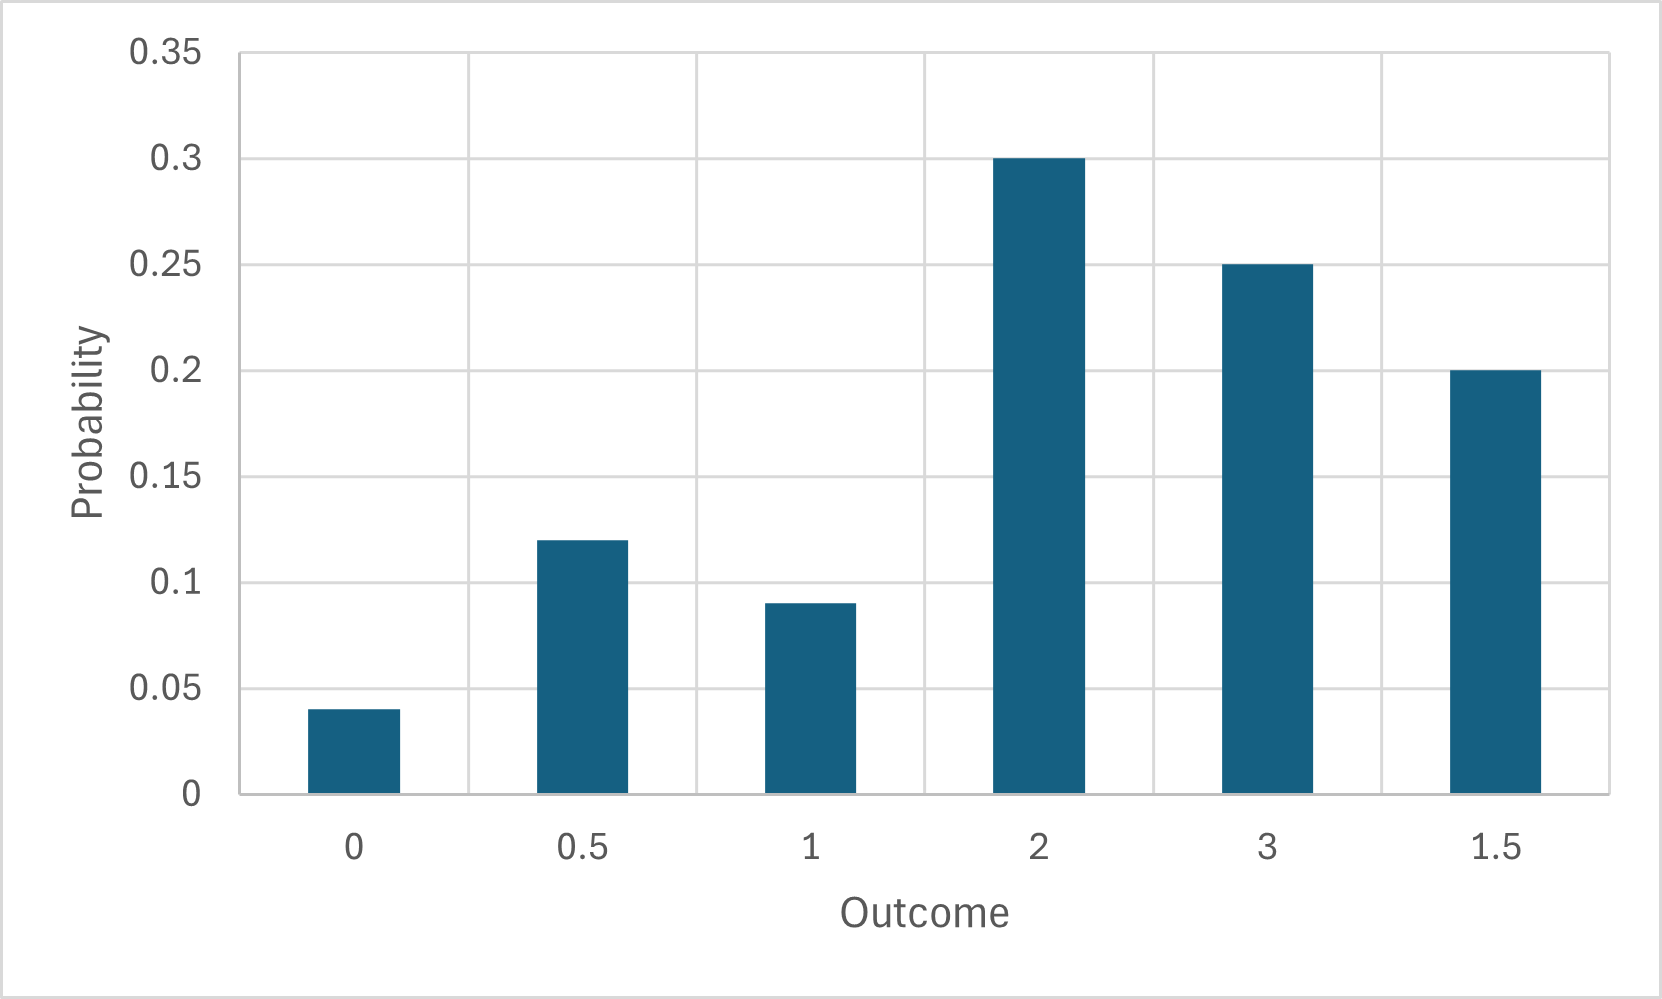
\includegraphics[keepaspectratio]{Picture/Picture1.png}}
                    \label{fig1}
                \end{figure}

            
        \item Determine $E[X_2]$ and $Var(X_2)$
        
        $\displaystyle E[X_2] = 1.8$

        $\displaystyle Var(X_2) = .78$

        \item Plot the probability mass function of the average of a sample size of 3. $X_3 = \frac{X_1+X_2+X_3}{3}$
        
        \begin{tabular}{|c|c|c|}
            \hline
            \textbf{Event} & \bf{$X_2$} & \textbf{Probability} \\
            \hline
            0,0,0 & 0 & 0.08 \\
            0,0,1 & 0.333333333 & 0.036 \\
            0,1,1 & 0.666666667 & 0.054 \\
            1,1,1 & 1 & 0.027 \\
            0,0,3 & 1 & 0.06 \\
            0,3,3 & 2 & 0.15 \\
            3,3,3 & 3 & 0.125 \\
            1,1,3 & 1.666666667 & 0.135 \\
            1,3,0 & 1.333333333 & 0.18 \\
            1,3,3 & 2.333333333 & 0.225 \\
            \hline
            \end{tabular}
        
            \begin{figure}[!htbp]
                \centerline{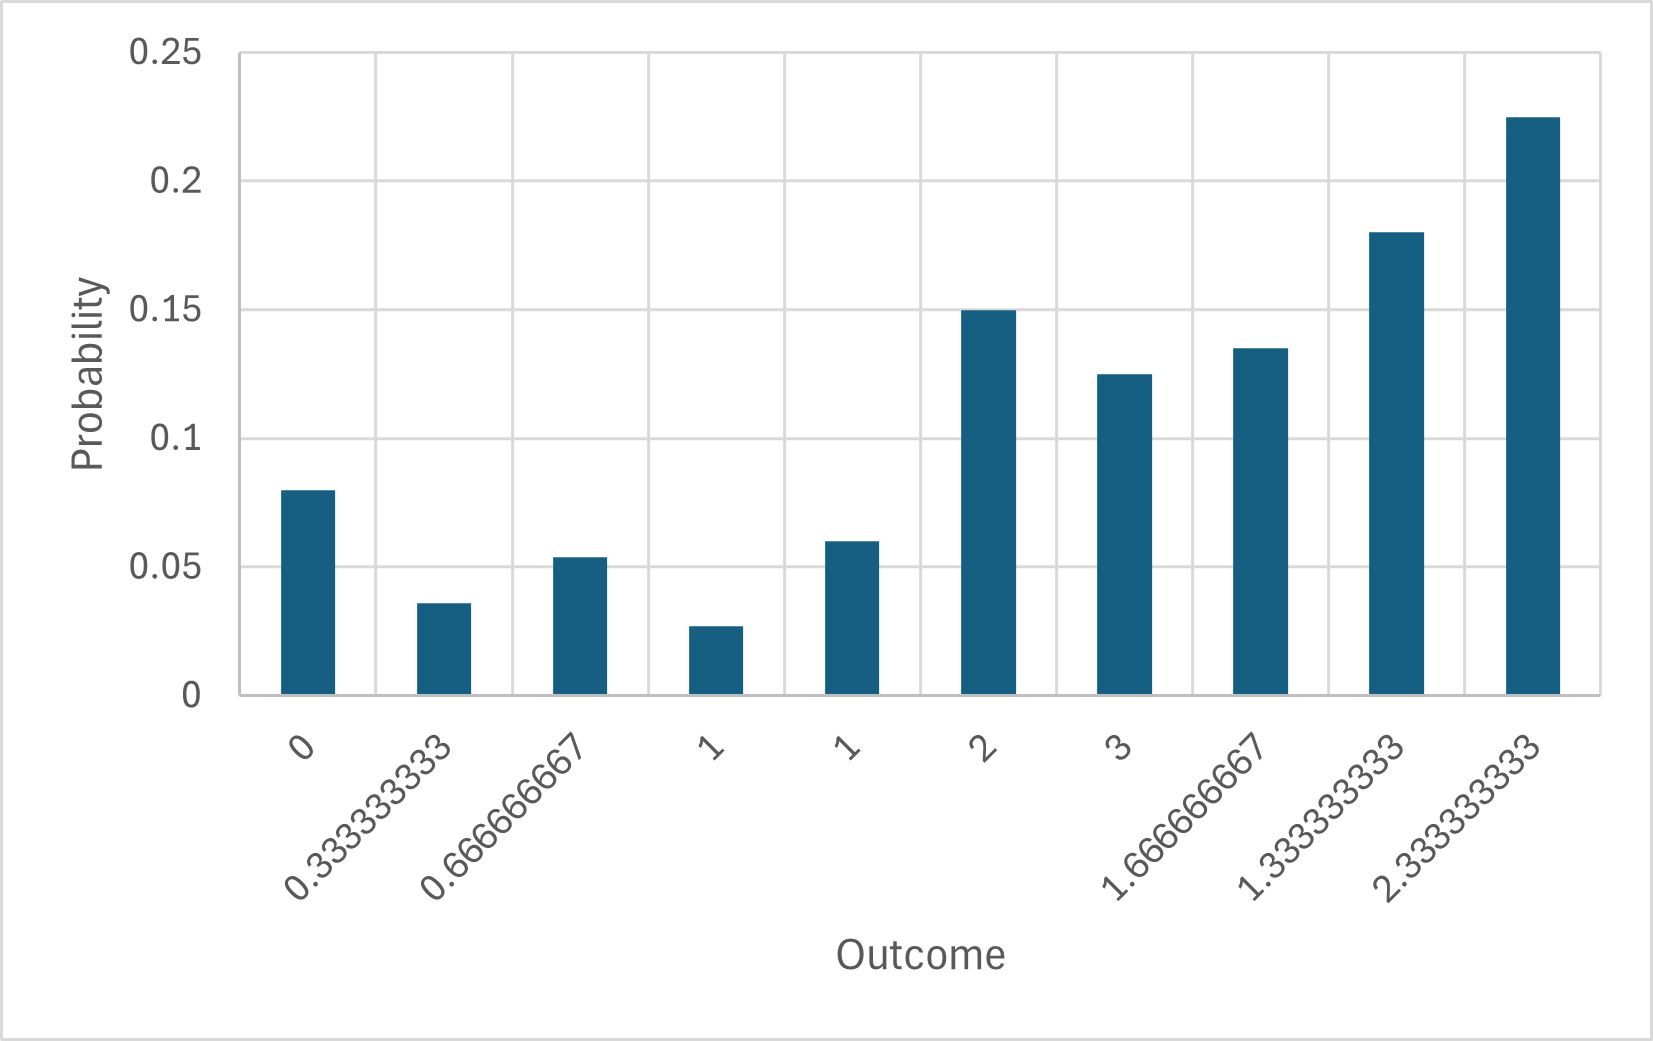
\includegraphics[keepaspectratio]{Picture/Picture2.png}}
                \label{fig1}
            \end{figure}
        \item Determine $E[X_3]$ and $Var(X_3)$
        
        $\displaystyle E[X_3] = 1.8$

        $\displaystyle Var(X_3) = 0.52$

    \end{enumerate}  
    \item If 10 fair dice are rolled, approximate the probability that the sum of the values obtained (which ranges from 10 to 60) is between 30 and 40 inclusive.
    
    Solution:

    $E[X_i] = \displaystyle \sum_{x_i = 1}^6 {\frac{1}{6}x = \frac{7}{2}}$

    $Var(X_i) = \displaystyle \sum_{x_i = 1}^6 {\frac{1}{6}{(x - \frac{7}{2})}^2 = \frac{35}{12}}$

    Let $X = \displaystyle \sum_{x_i = 1}^6 {X_i}$

    $E[X_i] = \displaystyle \sum_{x_i = 1}^{10} {E(X_i)} = 10(\frac{7}{5}) = 35$

    $Var(X_i) = \displaystyle \sum_{x_i = 1}^{10} {Var[X_i]} = 10(\frac{35}{12}) = \frac{350}{12}$

    $P(30 \leq X \leq 40) = P(29.5 < X < 39.5)$

    $= \displaystyle P\left(\frac{29.5 - 35}{\sqrt{350/12}}<\frac{X - 35}{\sqrt{350/12}}\frac{39.5 - 35}{\sqrt{350/12}}\right)$

    $= \displaystyle P\left(-1.02 \leq Z \leq 1.02 \right)$

    $= 2(0.8461)-1$

    $=0.6922$

    \item A highway department has enough salt to handle a total of 80 inches of snowfall. Suppose the daily amount of snow has a mean of 1.5 inches and a standard deviation of .3 inch.
    \begin{enumerate}
        \item Approximate the probability that the salt on hand will suffice for the next 50 days.
        
        Solution:
        
        Given:

        $E[X_i] = 1.5$ inches

        $SD[X_i] = 0.3$ inches

        Let $X = \displaystyle \sum_{x_i = 1}^{50} {X_i} $

        $E[X] = \displaystyle \sum_{x_i = 1}^{50} {E(X_i)} = 50(1.5) = 75$

        $Var(X) = \displaystyle \sum_{x_i = 1}^{50} {(SD[X_i])^2 = 50(0.09) = 4.5}$
    
        $\displaystyle P(X \leq 80) = P\left(\frac{X - 75}{\sqrt{4.5}}<\frac{80 - 75}{\sqrt{4.5}}\right)$

        $= \displaystyle P\left(\leq Z \leq 2.36 \right)$
    
        $=0.9908$
        \item What assumption did you make in solving part (a)?
        
        Solution:

        It is assumed that $X_i$ are independent and normal distributed random variables
        
        \item Do you think this assumption is justified? Explain briefly.
        
        Solution:

        This assumption is not justified because given snowfall in last few days is dependent on the atmospheric conditions, which would also affect today's rainfall.
    \end{enumerate}
    \item  The lifetime (in hours) of a type of electric bulb has expected value 500 and standard deviation 80. 
    Approximate the probability that the sample mean of n such bulbs is greater than 525 when
       
    Given:

        $E[X_i] = 500$ hours

        $SD[X_i] = 80$ hours

        Let $\bar{X_n} = \displaystyle \frac{\sum_{x_i = 1}^{50} {X_i}}{n}$
    
        $\displaystyle P(\bar{X_n} > 525) = P\left(\frac{\bar{X_{25}} - 500}{80/\sqrt{n}}<\frac{525 - 500}{80/\sqrt{n}}\right)$

        $= \displaystyle P\left(\leq Z > \sqrt{n}\frac{25}{80}\right)$
    
        $=1 - P\left(\leq Z = \sqrt{n}\frac{25}{80}\right)$

    \begin{enumerate}
        \item n = 4;

         $\displaystyle P(\bar{X_4} > 525) = 1 - P\left(\leq Z = \sqrt{4}\frac{25}{80}\right)$
         
         $= 1 - 0.7324$

         $= 0.2676$

        \item n = 16;

        $\displaystyle P(\bar{X_16} > 525) = 1 - P\left(\leq Z = \sqrt{16}\frac{25}{80}\right)$
        
        $= 1 - 0.8944$
        $= 0.1056$

        \item n = 36;

        $\displaystyle P(\bar{X_36} > 525) = 1 - P\left(\leq Z = \sqrt{36}\frac{25}{80}\right)$
        
        $= 1 - 0.9699$
        
        $= 0.0301$

        \item n = 64.

        $\displaystyle P(\bar{X_64} > 525) = 1 - P\left(\leq Z = \sqrt{64}\frac{25}{80}\right)$
        
        $= 1 - 0.9938$
        
        $= 0.0062$
    \end{enumerate}
    \item Fifty-two percent of the residents of a certain city are in favor of teaching evolution in high school. Find or approximate the probability that at least 50 percent of a random sample of size n is in favor of teaching evolution, when
    
    Given:

    $p = 0.52$

    $X_i = 
    \begin{cases}
    1, & \text{if } i^{th} \, \text{resident is in favour of teaching evolution},\\
    0, & \text{otherwise}\\
    \end{cases}$

    Let $X_n = \displaystyle \sum_{i=1}^n{X_i}$
    $P\left(X_n \geq \frac{n}{2}\right) = P\left(X_n > \frac{n}{2} - 0.5\right)$

    $= P\left(\frac{X_n - 0.52n}{\sqrt{0.2496n}} > \frac{n/2 - 0.5 - 0.52n}{\sqrt{0.2496n} \equiv a_n}\right)$

    $= P(Z > a_n)$

    \begin{enumerate}
        \item n = 10;
        
        $a_{10} = \frac{10/2 - 0.5 -0.52(10)}{\sqrt{0.2496(10)}}$

        $= -0.44$

        $P\left(X_n \geq \frac{n}{2}\right) = P\left(Z \leq 0.44\right)$

        $= 0.6711$
        \item n = 100;
        
        $a_{100} = \frac{100/2 - 0.5 -0.52(100)}{\sqrt{0.2496(100)}}$

        $= -0.5$

        $P\left(X_n \geq \frac{n}{2}\right) = P\left(Z \leq 0.5\right)$

        $= 0.6918$

        \item n = 1000;
        
        $a_{1000} = \frac{1000/2 - 0.5 -0.52(1000)}{\sqrt{0.2496(1000)}}$

        $= -1.3$

        $P\left(X_n \geq \frac{n}{2}\right) = P\left(Z \leq 1.3\right)$

        $= 0.9027$
        \item n = 10,000.
        
        $a_{10000} = \frac{10000/2 - 0.5 -0.52(10000)}{\sqrt{0.2496(10000)}}$

        $= -4.01$

        $P\left(X_n \geq \frac{n}{2}\right) = P\left(Z \leq 4.01\right)$

        $= .9997$
    \end{enumerate}

    \item An electric scale gives a reading equal to the true weight plus a random error that is normally distributed with mean 0 and standard deviation $\sigma$ = .1 mg. Suppose that the results of five successive weighings of the same object are as follows: $3.142, 3.163, 3.155, 3.150, 3.141$.
    $\displaystyle \bar{x} = \frac{\sum_{i}{x_i}}{n}$

    $= 3.1502$
    \begin{enumerate}
        \item Determine a 95 percent confidence interval estimate of the true weight.
        
        $\bar{x} - z_{0.025}\sigma/\sqrt{n} \leq \mu \leq \bar{x} + z_{0.025}\sigma/\sqrt{n}$

        $3.1502 - 1.96(0.1)/\sqrt{5} \leq \mu \leq 3.1502 + 1.906(0.1)/\sqrt{5}$

        $3.0625 \leq \mu \leq 3.2379$
        \item Determine a 99 percent confidence interval estimate of the true weight.
        
        $\bar{x} - z_{0.005}\sigma/\sqrt{n} \leq \mu \leq \bar{x} + z_{0.005}\sigma/\sqrt{n}$

        $3.1502 - 2.58(0.1)/\sqrt{5} \leq \mu \leq 3.1502 + 2.08(0.1)/\sqrt{5}$

        $3.0348 \leq \mu \leq 3.2656$
    \end{enumerate}

    \item  The following are scores on IQ tests of a random sample of 18 students at a large eastern university.
    $130, 122, 119, 142, 136, 127, 120, 152, 141, 132, 127, 118, 150, 141, 133, 137, 129, 142$
    
    if $X_i$'s are normally distributed, $\displaystyle t=\frac{\bar{X}-\mu}{S/\sqrt{n}}$ has $t$ distributed with $n-1$ degrees of freedom.

    $\displaystyle \bar{x} = \frac{\sum_{i}{x_i}}{n}$

    $= 133.22$
    
    $\displaystyle s^2=\sqrt{\frac{\sum_i{(x_i-\bar{x})^2}}{n-1}}$

    $= 10.2128$

    \begin{enumerate}
        \item Construct a 95 percent confidence interval estimate of the average IQ score of all students at the university
        
        $\bar{x} - z_{0.025}\sigma/\sqrt{n} \leq \mu \leq \bar{x} + z_{0.025}\sigma/\sqrt{n}$

        $133.22 - 2.11(10.2128)/\sqrt{18} \leq \mu \leq 133.22 + 2.11(10.2128)/\sqrt{18}$

        $128.141 \leq \mu \leq 138.30$

        $(128.141, 138.30)$
        \item Construct a 95 percent lower confidence interval estimate.
        
        $\mu \leq \bar{x} - z_{0.005}\sigma/\sqrt{n}$

        $\mu \leq 133.22 - 1.74(10.2128)/\sqrt{18}$

        $\mu \leq 129.03$

        $(-\infty, 129.03)$
        \item Construct a 95 percent upper confidence interval estimate.
        
        $\bar{x} + z_{0.025}\sigma/\sqrt{n} \leq \mu$

        $133.22 + 1.74(10.2128)/\sqrt{18} \leq \mu$

        $\mu \leq 137.41$

        $(137.41, \infty)$
    \end{enumerate}
    \item The capacities (in ampere-hours) of 10 batteries were recorded as follows:
    
    $140, 136, 150, 144, 148, 152, 138, 141, 143, 151$

    \begin{enumerate}
        \item Estimate the population variance $\sigma^2$.
        
        Solution: 

        Given:
        
        $n = 10$

        $\displaystyle s^2=\sqrt{\frac{\sum_i{(x_i-\bar{x})^2}}{n-1}}$

        $s^2 = 32.23$

        \item Compute a 99 percent two-sided confidence interval for $\sigma^2$.
        
        Solution: 

        $(n-1)\frac{s^2}{X_{0.005}^2} \leq \sigma^2 \leq (n-1)\frac{s^2}{X_{0.995}^2}$

        $\displaystyle 9\left(\frac{32.23}{23.59}\right) \leq \sigma^2 \leq 9\left(\frac{32.23}{1.73}\right)$

        $12.3 \leq \sigma^2 \leq 167.67$

        $(12.3, 153.83, 167.67)$

        \item Compute a value $v$ that enables us to state, with 90 percent confidence, that $\sigma^2$ is less than $v$.
        
        Solution: 

        $0 \leq \sigma^2 \leq (n-1)\frac{s^2}{X_{0.90}^2}$

        $0 \leq \sigma^2 \leq 9\left(\frac{32.23}{4.17}\right)$

        $0 \leq \sigma^2 \leq 69.6$

    \end{enumerate}
    \item Independent random samples are taken from the output of twomachines on a production line. 
    The weight of each item is of interest. From the first machine, a sample of size 36 is taken, with sample mean weight of 120 grams and a sample variance of 4.
    From the second machine, a sample of size 64 is taken, with a sample mean weight of 130 grams and a sample variance of 5.
    It is assumed that the weights of items from the first machine are normally distributed with mean $\mu_1$ and variance $\sigma^2$ and that the weights of items from the second machine are normally distributed with mean $\mu_2$ and variance $\sigma^2$ (that is, the variances are assumed to be equal). 
    Find a 99 percent confidence interval for $\mu_1 - \mu_2$, the difference in population means.
    
    Solution:

    Given:

    $n_1=36$

    Sample mean weight of first machine, $\bar{x_1} = 120$ grams
    
    Sample variance of first machine, $s_1^2 = 4$

    $n_2=64$

    Sample mean weight of first machine, $\bar{x_1} = 130$ grams
    
    Sample variance of first machine, $s_1^2 = 5$
    
    Let $\bar{X_1}$ and $\bar{X_2}$ be the random variables corresponding to sample mean of first and second machine respectively, respectively.

    $\displaystyle \frac{\bar{X_1 - \bar{X_2} - \left(\mu_1 - \mu_2\right)}}{S_p\sqrt{1/n_1 + 1/n_2}} \sim t_{n_1+n_2-2}$ where

    $\displaystyle S_p^2 = \frac{(n-1)(S_1)^2+(n_2-1)(S_2)^2}{n_1+n_2-2}$

    $= \displaystyle s_p^2=\frac{(n_1-1)(s_1)^2+(n_2-1)(s_2)^2}{n_1+n_2-2}$]
    
    $= \displaystyle \frac{35(4)+ 63(5)}{98}$

    $= 4.643$

    $s_p = 2.155$

    $\left(\bar{x_1} - \bar{x_2} - t_{0.005}s_p{\sqrt{1/n_1+1/n_2}}, \bar{x_1} - \bar{x_2} + t_{0.005}s_p{\sqrt{1/n_1+1/n_2}}\right)$

    $\left(120 - 130 - 2.627(2.155){(1/36+1/64)}, 120 - 130 + 2.627(2.155){(1/36+1/64)}\right)$

    $\left(-11.18, -8.82\right)$

    \item  To estimate $p$, the proportion of all newborn babies that are male, the gender of 10,000 newborn babies was noted. If 5106 of them were male, determine
   
    Solution:

    Given:

    $n=10,000$

    Sample probability for being a male, $\displaystyle \hat{p}=\frac{5106}{10000} = 0.5106$
    \begin{enumerate}
        \item a 90 percent and
        
        $(\hat{p} - z_{0.05}\sqrt{\hat{p}(1-\hat{p})/n}, \hat{p} + z_{0.05}\sqrt{\hat{p}(1-\hat{p})/n})$\

        $(0.5106 - 1.645\sqrt{0.5106(1-0.5106)/10000}, 0.5106 + 1.645\sqrt{0.5106(1-0.5106)/10000})$

        $(0.5023, 0.5188)$

        $0.5106 \pm 0.10$
        \item a 99 percent confidence interval estimate of $p$.
        
        $(\hat{p} - z_{0.05}\sqrt{\hat{p}(1-\hat{p})/n}, \hat{p} + z_{0.05}\sqrt{\hat{p}(1-\hat{p})/n})$\

        $(0.5106 - 2.58\sqrt{0.5106(1-0.5106)/10000}, 0.5106 + 2.58\sqrt{0.5106(1-0.5106)/10000})$

        $(0.5977, 0.5235)$

        $0.5106 \pm .013$
    \end{enumerate}
\end{enumerate}
\end{document}